\section{Problems with existing DAGs}
\subsection{Network synchronization}
When a node accepts a request to attach a transaction to the local StreamNet, it broadcasts the changes to neighboring StreamNet nodes. 
When the neighbors receives the update, it will follow the same principles to merge these changes and further broadcast the updates. 
If this update cannot be accepted by a large number of neighbors, the probability of its being accepted by the entire network is largely reduced.
There are several problems in this:
\begin{itemize}
	\item Issues with offline updates. Offline updates are implemented in StreamNet, but when offline nodes rejoin, 
              they will broadcast all local updates, but their local updates will only be accepted as a whole and will not be partially accepted \cite{iota_presentation}.
              Example of partial updates is shown in Figure~\ref{offline}.
	\item Existing DAGs are currently unable to guarantee strong consistency in the network environment.
\end{itemize}

\begin{figure*}[ht]
\begin{center}
	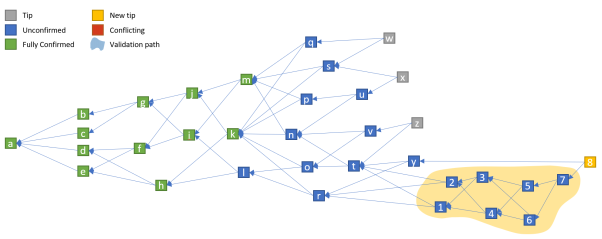
\includegraphics[width=0.65\textwidth]{figures/offline.png}
        \caption{Example of offline update \cite{iota_presentation} }
	\label{offline}
\end{center}
\end{figure*}

\begin{figure*}[ht]
\begin{center}
	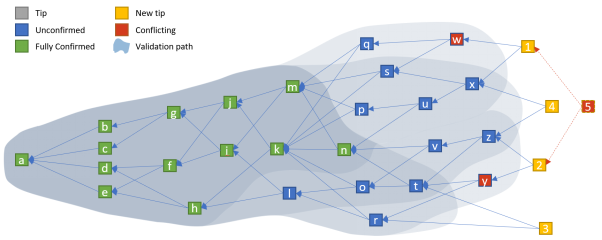
\includegraphics[width=0.65\textwidth]{figures/double_spend.png}
	\caption{Example of double spending problem}
	\label{double_spend}
\end{center}
\end{figure*}

\subsection{Double Spending Problem}
The double spending problem refers to the problem that the same token is used multiple times, which is shown in the example in Figure~\ref{double_spend}, 
where the two transactions of $w$ and $y$ are double spending transactions, and the transaction $5$ is the one that finds it out.
Given a confidence level (say 95\%) in the random walk algorithm, 
one of the transactions will naturally receive more transaction approvals in the natural state until it reaches a state sufficient to be confirmed.
For example, as shown in Figure~\ref{double_spend}, $w$ receives more confirmations in the future, and slowly $y$ is isolated to lose the possibility of being confirmed later. 
But when the fraudster's power is strong enough, it can issue enough transactions to approve $w$ after a transaction is confirmed, then in this case, the previously confirmed transaction will in turn be marginalized.
To achieve the purpose of double-spending, it is necessary to accumulate $34\%$ of the computing power of the whole network to achieve the goal \cite{popov2016tangle}. 
However, considering the low number of transactions in the entire network in the early stage, 34\% of the power attack is actually not difficult.
To solve this problem, the concept of coordinator is introduced, the transaction confirmed by the coordinator is absolutely valid.
Regardless of the computing power of the follow-on attacker, it can not beat the coordinator's one-vote veto . 
The introduction of coordinator is a centralized solution, and in the future, as more and more devices join the StreamNet network,
how to remove it to turn DAG into a decentralized network is a challenge.

\subsection{transaction confirmation speed problem}

\begin{figure}[!ht]
\begin{center}
	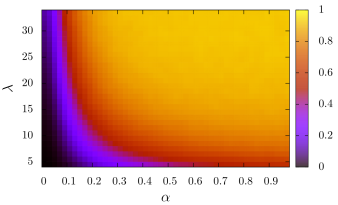
\includegraphics[width=0.35\textwidth]{figures/alpha.png}
        \caption{The probability of a transaction being permanently stuck (failed), $\alpha$ is randomness, $\lambda$ is the transaction rate \cite{iota_confirm}}
	\label{iota_confirm}
\end{center}
\end{figure}

\begin{figure*}[!ht]
\begin{center}
	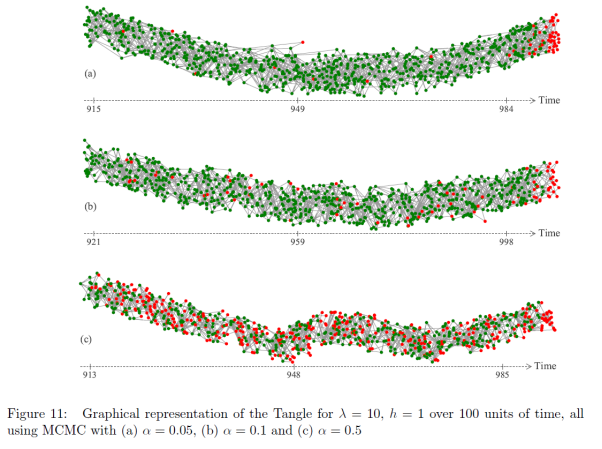
\includegraphics[width=0.75\textwidth]{figures/dagvis.png}
	\caption{A more intuitive expression of the role}
	\label{dagvis}
\end{center}
\end{figure*}

The speed at which the transaction is confirmed and the likelihood that the transaction will be finalized depends on two factors, the first is the transaction rate $\lambda$, and the second is the randomness $\alpha$. 
From Figure~\ref{iota_confirm}, it can be seen that the probability of increasing the success of the transaction is mainly due to the increase the $\lambda$ and reduces $\alpha$. 
and in Figure~\ref{iota_confirm}, a more intuitive expression of the effect of $\alpha$ can be seen in Fifure~\ref{dagvis}, under the same conditions, the higher $\alpha$ will result in more unconfirmed transactions.
However, because the transaction rate in the whole network is relatively slow, there are not many active nodes, thus some ad-hoc optimization methods have been proposed.
For example, the method of coordinator mentioned before and the method of Reattach, rebroadcast etc. 

\subsection{Encryption Algorithm Vulnerabilities}
Because the current DAG encryption algorithm is based on Trytes, 
and the encryption algorithm is invented from scratch, the method pointed out in \cite{iota_collision} can find the hash collision in a few minutes using commodity hardware. 
The attacker can use this vulnerability to fake other users. Signature, fundamentally disintegrating the security of IOTA.

\subsection{ replay attack}
Replay attacks In addition to the use of power to attack in the double-spending problem, 
two attack modes are mentioned in the white paper, the first one is a side chain attack and the other is a double-sided chain attack \cite{iota_proof}. 

